% ICLR 2027 draft. Compiles with the official style if iclr2027_conference.sty/.bst sit in
% this directory (https://media.iclr.cc/Conferences/ICLR2027/iclr-2027-style-files.zip);
% otherwise falls back to article so the draft builds today. Build:
%   latexmk -pdf -interaction=nonstopmode main.tex
% Every "\keypoints" box lists what the section must land; delete the boxes before
% submission. "\todo" marks numbers or claims still to be produced.
\documentclass{article}
\IfFileExists{iclr2027_conference.sty}{%
  \usepackage{iclr2027_conference,times}%
  % \iclrfinalcopy  % uncomment for camera-ready
}{%
  \usepackage[margin=1in]{geometry}%
  \usepackage{times}%
}
\usepackage{natbib}
\usepackage{amsmath,amssymb,amsthm}
\usepackage{booktabs,array,multirow}
\usepackage{graphicx}
\usepackage{xcolor}
\usepackage{enumitem}
\usepackage{algorithm,algorithmic}
\usepackage{hyperref}
\usepackage[nameinlink,noabbrev]{cleveref}
\graphicspath{{./figures/}{../gas-mpc/}}

\newcommand{\z}{z}
\newcommand{\psiT}{\psi}
\newcommand{\Htd}{H_{\mathrm{TD}}}
\newcommand{\ET}{\mathrm{ET}}
\newcommand{\todo}[1]{\textcolor{red}{[TODO: #1]}}
\newcommand{\keypoints}[1]{\par\medskip\noindent\fcolorbox{black!50}{black!5}{\begin{minipage}{0.96\linewidth}\small
\textbf{Key points this section must land.}\begin{itemize}[nosep,leftmargin=1.2em]#1\end{itemize}\end{minipage}}\par\medskip}

\title{Graph-Guided Long-Horizon MPC with World Models}
\author{Anonymous authors\\Paper under double-blind review}

\begin{document}
\maketitle

\begin{abstract}
The cross-entropy method (CEM) planner used with LeWorldModel (LeWM) ranks candidate action
sequences by the Euclidean distance between a predicted terminal latent and a goal latent. While
this objective succeeds on short-horizon goals, its performance degrades sharply as goals become
more temporally distant or come from a different episode. On Push-T, the planner reaches
same-episode goals 25, 50 and 100 steps ahead, and cross-episode goals, with success rates of
91/41/13/14\%, respectively. We address this degradation at long horizons and across episodes
without retraining the world model or learning a subgoal generator. We learn a temporal
distance representation over frozen latents, build a graph of the offline dataset, and use
shortest paths to select a data-supported subgoal one planning horizon ahead. A budget-clocked
expected-hitting-time critic scores predicted endpoints by time to goal under the remaining
budget, and the planner switches back to latent L2 for the final horizon. Each component addresses a distinct
limitation: the subgoal provides \emph{direction}, the critic accounts for \emph{feasibility},
and the final switch restores near-goal \emph{resolution}. Across fixed task pools and five seeds,
our method raises success from 41/13/14\% to 70/46/42\% on Push-T and from 91/83/29\% to
98/98/66\% on Reacher at offsets 50, 100 and cross-episode. At the
25-step horizon, however, it does not outperform L2, trailing by 3 percentage points on Push-T and
1 point on Reacher. Per-pair diagnostics show that the graph contains routes for all evaluated
cross-episode pairs, but executing them requires the feasibility critic.
\end{abstract}

% =====================================================================================
\section{Introduction}
\keypoints{
\item The problem is the \emph{objective}, not the model: terminal latent L2 stops ranking
      candidates past $\sim$50 steps and is blind to cross-episode goals (10\% at any budget).
\item Existing fixes retrain the encoder, add predictors, or learn generators. We keep the
      world model and its planner frozen and use the dataset itself as a graph.
\item Three mechanisms, three failures: direction (graph subgoal), feasibility (hitting-time
      critic), resolution (final switch). Neither subgoal nor critic alone moves cross-episode.
\item Cross-episode goal reaching is the headline evaluation; same-episode long horizons are
      supporting evidence.
\item Contributions list, four items, each tied to a table or figure.
}

Joint-embedding world models trained from pixels \citep{lewm,dinowm,pldm} plan by search:
sample action sequences, roll them through a learned latent predictor, and keep the sequences
whose predicted terminal latent is closest to the goal latent. On the benchmarks these models are
evaluated on, the goal is a frame from the same trajectory a fixed number of steps ahead, and the
planner is very good at it. It is much less good at anything further away. With the frozen
LeWorldModel (LeWM) checkpoint and its published cross-entropy-method (CEM) planner, Push-T
success is 91\% for goals 25 steps ahead, 48\% at 50 steps, 11\% at 100 steps, and 10\% for a
goal drawn from a different episode, a number that does not move when the budget is raised from
25 to 250 steps (\cref{sec:problem}).

The failure is in the objective. A privileged audit shows the terminal latent distance ranks
candidate endpoints well at 25 steps (Spearman 0.72 against a recovery-time oracle) and poorly at
50 (0.36); a single-pass audit shows the predicted terminal cost is optimistic on 88\% of tasks
and barely separates successes from failures (\cref{sec:problem}). The planner is not wrong about
where the goal is; it is wrong about which of its candidates can still get there.

A wave of recent work attacks the same failure on the same frozen model, and almost all of it
learns something new on top: a subgoal generator and action prior \citep{sage}, a macro-action
space and high-level predictor \citep{hilewm}, world models at several time scales \citep{hwm},
an action-free latent planner \citep{ffjepa}, or a retrained encoder whose geometry encodes
temporal cost \citep{tdjepa,rcaux,trm}. A separate, older line in offline goal-conditioned RL
answers long horizons by \emph{search over the data}: build a graph over the offline dataset and
let shortest paths choose subgoals \citep{sptm,sorb,sgm,gas,ttgs,alps}. Those methods hand the
subgoal to a learned goal-conditioned policy. Nobody has put the dataset graph inside a pixel
world model's planner, and \citet{hilewm} explain why one might want to: their hierarchical
planner fails whenever its generated subgoals stop being ``data-supported, executable, and
matched to the temporal scale''. A subgoal that is a dataset frame is all three by construction.

This paper does that. We learn a temporal distance representation (TDR) on the frozen LeWM
latents \citep{hilp,gas}, build a graph over the full offline dataset in that space, and replace
LeWM's terminal cost with the distance to the graph node one planning horizon along the shortest
path to the goal. That alone repairs the mid-range regime (Push-T offset 50: $48\to61\%$) and
does nothing for cross-episode goals: by the graph's own geodesic every cross-episode pair is
45--120 steps apart, inside the budget, yet the planner does not execute the route. The missing
piece is feasibility. We add a critic $V(\z,\z_g,h)$, the probability that the goal is reachable
from latent $\z$ within $h$ steps, and score each predicted endpoint by a budget-capped
\emph{expected hitting time} under the steps that remain after the plan being scored. With that
term, and with the final horizon handed back to LeWM's own objective once the goal is one horizon
away, a single configuration is at or above every alternative on every protocol we tested
(\cref{tab:main}).

Our contributions are:
\begin{enumerate}[nosep,leftmargin=*]
  \item A planner-side method for long-horizon and cross-episode goal reaching with a frozen
        pixel world model that trains no generator, no policy and no new predictor: a TDR on
        frozen latents, a dataset graph, a hitting-time critic, and one unchanged CEM
        (\cref{sec:method}).
  \item A budget-clocked expected-hitting-time cost that replaces the usual $-\log V$ feasibility
        term, removes its weight dependence, and keeps a progress gradient among feasible
        candidates (\cref{sec:critic,sec:ablation}).
  \item The first cross-episode goal-reaching evaluation for latent MPC on Push-T, Reacher and
        \todo{Cube}, with fixed task pools shared by every method and seed (\cref{sec:setup}).
  \item A mechanistic account, with per-pair diagnostics, of which failure each component
        repairs: direction, feasibility, and resolution (\cref{sec:analysis}).
\end{enumerate}

% =====================================================================================
\section{Related work}
\label{sec:related}
\keypoints{
\item Group by what is learned, not by year: (i) planner-side costs on a frozen model,
      (ii) hierarchical planning with learned generators/predictors, (iii) graph search over
      offline data with learned policies, (iv) value functions inside MPC.
\item For each group say in one clause what we take and in one clause what we do not.
\item Be explicit that SAGE reports higher same-episode numbers at $H\!=\!150$ and cannot stitch
      by construction; do not hide it, it is our argument.
}

\paragraph{Planning with latent world models.}
PlaNet and Dreamer \citep{planet,dreamerv3} plan or learn policies in a reconstruction-based
latent; DINO-WM \citep{dinowm}, PLDM \citep{pldm}, V-JEPA~2-AC \citep{vjepa2} and LeWM
\citep{lewm} plan with zero-shot CEM in a joint-embedding latent, scoring candidates by terminal
latent distance. \citet{jepawm-study} and \citet{stableworldmodel} study which design choices
matter; the planning horizon is a known weak point of all of them.

\paragraph{Repairing the cost on a frozen model.}
Trajectory reachability metrics \citep{trm} learn a pairwise temporal cost from logged
trajectories and use it as the terminal ranking; temporal-distance JEPA \citep{tdjepa},
RC-aux \citep{rcaux}, DA-LeWM \citep{dalewm} and SCALE \citep{scale} push similar signals into
the encoder at training time, and \citet{valueguided,straightening} shape the geometry toward a
value or a straight path. Our TDR is in the same family (an expectile temporal distance on frozen
latents) but we do not use it as the cost: we use it to build a graph and pick a data-supported
target, and we show the metric alone is not what helps (\cref{sec:ablation}). RC-aux's
budget-conditioned reachability is the closest relative of our critic; ours is a separate
network with an explicit plan clock and never touches the encoder.

\paragraph{Hierarchical planning with world models.}
HWM \citep{hwm} learns world models at several temporal scales and uses long-horizon predictions
as subgoals; SAGE \citep{sage} learns a subgoal generator and a subgoal-conditioned action prior
that CEM refines; FF-JEPA \citep{ffjepa} learns an action-free latent planner; Hi-LeWM
\citep{hilewm} learns macro-actions and a high-level predictor and shows the naive version loses
to flat planning because CEM exploits the learned subgoal space. Each of these trains a generative
component whose training pairs are same-trajectory windows, so their subgoals cannot lie on a
route that no single trajectory took. Our subgoals are dataset frames on a shortest path over
the whole dataset, and the cross-episode protocol is where that difference shows. SAGE reports
stronger same-episode numbers than ours at long offsets (64.7\% at $H\!=\!150$ on Push-T with the
same frozen model); we discuss this in \cref{sec:limitations}.

\paragraph{Graph search over offline data.}
SPTM \citep{sptm}, SoRB \citep{sorb} and SGM \citep{sgm} build graphs over replay buffers with a
learned distance and plan waypoints for a goal-conditioned policy; GAS \citep{gas} clusters a
temporal distance representation \citep{hilp,qrl} into nodes with a temporal-efficiency filter and
searches it for subgoals; TTGS \citep{ttgs} and ALPS \citep{alps} do the same at test time for
frozen OGBench policies \citep{ogbench}. All of them execute subgoals with a learned policy (or a
state-space model with a behaviour prior). We take GAS's graph construction essentially unchanged
and give the subgoal to a pixel world model's CEM instead; an earlier RL version of GAS on the
same latent found the low-level policy, not the graph, to be the win, which is why the executor
matters and why we test it separately.

\paragraph{Value functions inside MPC.}
POLO \citep{polo}, TD-MPC \citep{tdmpc,tdmpc2} and Director \citep{director} put a learned value
at the end of a short model rollout; goal-conditioned terminal values have been used for
multi-task MPC \citep{gcterminal}. Those values are trained with rewards or with the model. Our
critic is a reachability classifier trained from hindsight and cross-episode negatives on the
offline data, and its contribution is a budget-aware hitting time rather than a value.

% =====================================================================================
\section{The problem: latent MPC beyond one horizon}
\label{sec:problem}
\keypoints{
\item Define the planner exactly once (300 samples, 30 iterations, 30 elites, 5 blocks of 5
      actions, open-loop 25 steps, replan). Everything downstream changes only the criterion.
\item Two audits, one figure: (a) oracle Spearman of terminal L2 vs recovery time drops
      $0.72\to0.36$ from offset 25 to 50; (b) single-pass predicted vs realized terminal cost:
      optimistic on 88.5\% of tasks, Spearman 0.30, medians 2.2 vs 2.3 (pred) against 11 vs 30 (real).
\item Cross-episode is flat in budget: 4/8/9/11\% at 25/50/100/175+ steps.
}

\paragraph{Frozen world model and planner.}
LeWM \citep{lewm} consists of a ViT encoder $E$ mapping a $224\times224$ frame to a 192-d CLS
latent $\z$ and a predictor $P$ that maps three past latents and three action blocks to the next
latent, where an action block is five consecutive environment actions (frame-skip 5). Planning is
CEM over $K=5$ blocks (25 environment steps): 300 candidates, 30 iterations, 30 elites, each
candidate scored by the terminal cost $c_{\mathrm{L2}}=\|\hat\z_K-\z_g\|^2$ between the predicted
block-$K$ latent and the encoded goal frame. The optimum is executed open loop for 25 steps and
the planner is called again. We keep the encoder, the predictor and this planner fixed
throughout and change only the function that scores $(\z_0,\hat\z_{1..K},\z_g)$.

\paragraph{Where it fails.}
\Cref{tab:main} (rows ``L2'') gives the picture on three environments: near-perfect one horizon
out, a steep fall past two, and a floor for goals from another episode. Two audits locate the
failure in the ranking. First, against a privileged recovery-time oracle (the number of steps a
strong planner with state access needs from a candidate endpoint), $c_{\mathrm{L2}}$ orders
endpoints with Spearman 0.72 at offset 25 and 0.36 at offset 50. Second, executing the single
25-step plan of 200 offset-25 tasks and re-encoding the true final frame, the predicted cost
under-estimates the realized latent distance on 88.5\% of tasks, correlates with it at only
$\rho=0.30$, and barely separates successes from failures (median 2.17 vs 2.31) while the realized
distance does (10.9 vs 30.0; \cref{fig:single-pass}). The planner optimises a quantity that is
optimistic and, past one horizon, uninformative about which endpoints can still reach the goal.
Cross-episode success is 4.4/7.6/8.8/10.8\% at budgets 25/50/100/175+: more time does not help.

\begin{figure}[t]
  \centering
  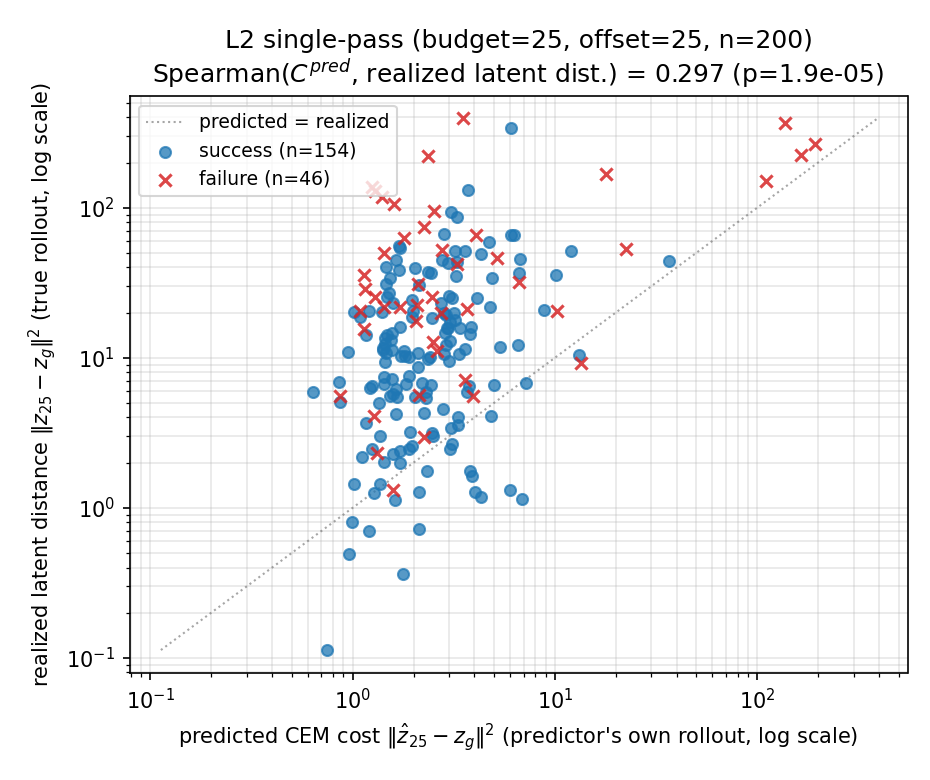
\includegraphics[width=0.5\linewidth]{fig_l2_single_pass_predicted_vs_realized}
  \caption{Single-pass L2 CEM on 200 offset-25 Push-T tasks: predicted terminal cost from the
  predictor's own rollout against the realized latent distance of the executed plan (both log
  scale). Points above the dotted identity line are optimistic predictions (88.5\%).
  \todo{Replace with a two-panel figure: (a) this; (b) the ablation ladder across protocols.}}
  \label{fig:single-pass}
\end{figure}

% =====================================================================================
\section{Method}
\label{sec:method}
\keypoints{
\item One equation per component. The reader should be able to reimplement from the section.
\item Say what is learned (TDR: 3$\times$512 MLP; critic: 5-member MLP ensemble) and what is
      not (encoder, predictor, CEM, graph is built not trained).
\item State the privileged-label dependency of the critic here, in the open.
\item The plan clock: $h_{\mathrm{rem}}$ is the budget left \emph{after} the plan being scored.
      This is the single most important implementation detail.
\item Only two scalars are environment specific ($\Htd$, $\lambda$) and both are read off the
      TDR's own step-gap calibration; $\beta=1$ everywhere.
}

\subsection{Temporal distance representation and dataset graph}
\label{sec:graph}
We encode every frame of the offline dataset once with the frozen encoder and train a small MLP
$\psiT:\mathbb{R}^{192}\to\mathbb{R}^{32}$ so that $\|\psiT(\z)-\psiT(\z_g)\|$ approximates the
minimum number of steps from $\z$ to $\z_g$, using the expectile temporal-difference objective of
HILP and GAS \citep{hilp,gas} (expectile 0.99, $\gamma=0.99$, goals relabelled from the same
trajectory with probability 0.625 and uniformly otherwise). We calibrate what one TDR unit means by
the median TDR distance between frames $k$ steps apart, $u_k$, for $k\in\{1,\dots,50\}$; this table
is the only place environment scale enters.

The graph follows GAS: frames whose temporal efficiency (the ratio of TDR progress to steps
taken) falls below $\theta_{\mathrm{TE}}=0.9$ are dropped, the rest are clustered sequentially in
TDR space at radius $\Htd/2$, and nodes within $\Htd$ of each other are joined by edges weighted by
TDR distance. $\Htd$ is $u_{12}$, the TDR distance of a 12-step gap. Each node stores its medoid
frame's latent. At planning time the goal latent is attached as a temporary node linked to every
node within $\max(\Htd,1.2\,d_{\min})$ and one Dijkstra pass gives $D_g[v]$, the cost-to-go from
every node. On Push-T (18{,}685 expert episodes, 2.34M frames) the graph has 20.5k nodes;
Reacher (10k episodes, 2.01M frames) needs 535; \todo{Cube}. Building it is a one-off cost of
\todo{x} minutes on one GPU.

\subsection{Subgoal one horizon ahead, and the final switch}
\label{sec:subgoal}
At each planning call with current latent $\z_0$, we select the start node
$v^\star=\arg\min_{v:\|\psiT(\z_0)-c_v\|\le\Htd} D_g[v]+\|\psiT(\z_0)-c_v\|$ and walk the shortest
path from $v^\star$ toward the goal until the cumulative TDR distance from $\z_0$ reaches the
lookahead $\lambda=u_{25}$, the calibrated distance of one planning horizon. The node reached,
$v_\lambda$, is the subgoal and the criterion becomes
\begin{equation}
  c_{\mathrm{sub}}(\hat\z_K)=\|\psiT(\hat\z_K)-c_{v_\lambda}\|.
  \label{eq:subgoal}
\end{equation}
Placing the subgoal exactly one horizon out matters: shorter lookaheads leave progress on the
table and waypoint tracking over the intermediate predicted latents is worse than the terminal
cost alone (\cref{sec:ablation}), because those latents are the predictor's least reliable
outputs. Once the goal itself is within one horizon, $\|\psiT(\z_0)-\psiT(\z_g)\|\le\lambda$, the
criterion reverts to LeWM's own $c_{\mathrm{L2}}$ against the true goal frame. This
\emph{final switch} is what lets the method reduce to the baseline wherever the baseline is best:
a cluster medoid has a radius comparable to the success tolerance, and the TDR norm has less
resolution at the goal than the latent L2.

\subsection{Budget-clocked expected hitting time}
\label{sec:critic}
A reachability critic $V(\z,\z_g,h)\in[0,1]$ estimates the probability that the goal can be reached
from latent $\z$ within $h$ environment steps. It is a five-member MLP ensemble on
$(\z,\z_g,h)$ with $h$ on a grid of multiples of 5 up to $h_{\max}=50$, trained on the offline
dataset with (i) hindsight labels $\mathbb{1}[h\ge\tau]$ where $\tau$ is the first step at which
the logged trajectory satisfies the environment's success predicate toward a later frame, (ii)
cross-episode negatives whose object or joint configuration differs by more than the data ever
moves in 50 steps, (iii) predictor-imagined rollouts under logged actions, (iv) a Bellman backup
through the frozen predictor with an EMA target aggregated pessimistically, and (v) a hinge
enforcing monotonicity in $h$. The labels in (i) and the gate in (ii) evaluate the success
predicate on the dataset's state column; the critic's inputs are latents only, but its training
is not pixel-only, and we return to this in \cref{sec:limitations}.

Rather than the usual $-\log V$ penalty, we score an endpoint by how long the goal is expected to
take from it, capped at the budget that will remain once the plan being scored has been executed:
\begin{equation}
  \ET(\hat\z_K)=5\sum_{h\in\{0,5,\dots,h_{\mathrm{rem}}\}}\big(1-V(\hat\z_K,\z_g,h)\big),
  \qquad h_{\mathrm{rem}}=\min\big(h_{\max},\,B-t-5K\big),
  \label{eq:et}
\end{equation}
where $B$ is the episode budget and $t$ the current step. A \emph{plan clock} supplies $t$: every
CEM call advances all live environments by one horizon, so the critic always answers ``reachable
in the steps that are left'' rather than at a fixed horizon. Feasible endpoints are ordered by how
soon they arrive; infeasible ones sit at the cap. The final criterion standardises both terms by
median and interquartile range over the 300 CEM candidates of each environment and adds them,
\begin{equation}
  c=\widetilde{c_{\mathrm{sub}}}+\beta\,\widetilde{\ET},\qquad \beta=1,
  \label{eq:compose}
\end{equation}
with $c_{\mathrm{L2}}$ in place of $c_{\mathrm{sub}}$ in the final phase. \Cref{alg:main}
summarises one planning call.

\begin{algorithm}[t]
\caption{One planning call of graph-assisted latent MPC}
\label{alg:main}
\begin{algorithmic}[1]
\REQUIRE frozen $E,P$; CEM; TDR $\psiT$; graph $(V_G,c_v,D_g)$; critic $V$; budget $B$; step $t$
\STATE $\z_0\gets E(o_t)$; \ $h_{\mathrm{rem}}\gets\min(h_{\max},B-t-5K)$
\IF{$\|\psiT(\z_0)-\psiT(\z_g)\|\le\lambda$} \STATE target $\gets$ goal; base cost $\gets c_{\mathrm{L2}}$
\ELSE \STATE $v^\star\gets\arg\min_{v:\|\psiT(\z_0)-c_v\|\le\Htd} D_g[v]+\|\psiT(\z_0)-c_v\|$
\STATE walk the shortest path from $v^\star$ until cumulative TDR distance $\ge\lambda$; target $\gets v_\lambda$; base cost $\gets c_{\mathrm{sub}}$
\ENDIF
\FOR{each CEM iteration}
  \STATE sample 300 action-block sequences; $\hat\z_{1..K}\gets P(\cdot)$
  \STATE $c\gets\widetilde{\text{base}}(\hat\z_K)+\widetilde{\ET}(\hat\z_K)$ with $\ET$ from \cref{eq:et}
  \STATE refit the CEM Gaussian on the 30 lowest-$c$ candidates
\ENDFOR
\STATE execute the mean sequence for $5K$ steps; $t\gets t+5K$
\end{algorithmic}
\end{algorithm}

\paragraph{What is learned, what is not.}
The TDR (50k steps, batch 1024) and the critic (60k steps) are the only trained components;
together they are under \todo{x}M parameters and take \todo{x} GPU-hours per environment. The
encoder, predictor, CEM hyperparameters and the graph-construction rules are LeWM's and GAS's,
unchanged. Two scalars are environment specific, $\Htd=u_{12}$ and $\lambda=u_{25}$, and both are
read off the TDR calibration table rather than tuned; $\beta=1$, $\theta_{\mathrm{TE}}=0.9$ and
$h_{\max}=50$ are shared by every environment and protocol.

% =====================================================================================
\section{Experiments}
\label{sec:experiments}

\subsection{Setup}
\label{sec:setup}
\keypoints{
\item Fixed task pools: 200 (start, goal) pairs per protocol per environment drawn once and shared
      by every method and seed; a ``seed'' changes CEM's draws (and, where stated, the learned
      assets), never the tasks. State how many of the 200 each table uses.
\item Protocols: same-episode offset $K\in\{25,50,100,150\}$ with budget $2K$ (cap 250);
      cross-episode with budget 250 (Push-T), 200 (Reacher), \todo{Cube}.
\item Success is the environment's own predicate. Say it for each environment.
\item Baselines: L2 (LeWM); L2 with more search; TDR-only cost; graph cost-to-go; oracle
      subgoal; \todo{TRM-style learned cost; SAGE}. Random floor.
}

\paragraph{Environments and data.}
Push-T \citep{lewm}: 18{,}685 expert episodes; success when agent and block position errors are
below 20\,px and block angle error below $\pi/9$. Reacher (dm\_control): 10{,}000 episodes of 201
frames; success when both joints are within 0.05\,rad of the goal configuration (raw difference,
no angle wrap; the dataset's shoulder angle is unwrapped over $\pm8$\,rad). OGBench Cube
\citep{ogbench}: 10{,}000 episodes of 201 frames; \todo{success predicate as scored}. Frozen LeWM
checkpoints are the public ones for each environment. \todo{Two-Room.}

\paragraph{Protocols.}
For a same-episode offset $K$, the goal is the frame $K$ steps after the start on the same
trajectory and the budget is $2K$ steps. For the cross-episode protocol the start and goal are
uniformly random frames of two different episodes with no distance or reachability filter and a
budget of one full episode. We draw 200 tasks per protocol once and use the same pool for every
method and every seed; unless stated, tables use the first 50 tasks and five CEM seeds (250
task-seed pairs per cell). Learned assets (TDR, graph, critic) use seed 0 unless stated;
\cref{app:seeds} separates asset seeds from CEM seeds.

\paragraph{Baselines.}
\emph{L2} is LeWM's planner. \emph{TDR} scores endpoints by $\|\psiT(\hat\z_K)-\psiT(\z_g)\|$ with no
graph; \emph{CTG} uses the graph cost-to-go $\min_v\|\psiT(\hat\z_K)-c_v\|+D_g[v]$ as a terminal value
with no subgoal commitment. \todo{L2 with double horizon and search budget; oracle subgoal (true
$+25$ frame); TRM-style learned pairwise cost; SAGE if code is released; random-policy floor.}

\subsection{Main result}
\label{sec:main}
\keypoints{
\item One table, three (four) environments, L2 vs the full method, four protocols, mean$\pm$sd over
      seeds plus pooled hits. Bold the winner only where the paired difference is significant.
\item The sentence to write: same at one horizon, better at two, much better beyond, and
      $4\times$ / $2.6\times$ on cross-episode, every seed.
}

\begin{table}[t]
\centering\small
\caption{Success rate (\%) on the fixed task pools, first 50 tasks, mean $\pm$ sd over five CEM
seeds (250 task-seed pairs per cell). Same tasks, CEM and predictor for both rows. Cube is
partial (\todo{seeds in progress}).}
\label{tab:main}
\begin{tabular}{llrrrr}
\toprule
Env & Method & same-ep 25 & same-ep 50 & same-ep 100 & cross-ep \\
\midrule
\multirow{2}{*}{Push-T} & L2 (LeWM) & \textbf{91.2} $\pm$ 3.0 & 48.4 $\pm$ 4.6 & 11.2 $\pm$ 2.0 & 10.4 $\pm$ 3.4 \\
 & Ours & 90.8 $\pm$ 2.7 & \textbf{64.4} $\pm$ 4.6 & \textbf{50.4} $\pm$ 5.0 & \textbf{44.4} $\pm$ 3.9 \\
\midrule
\multirow{2}{*}{Reacher} & L2 (LeWM) & \textbf{86.8} $\pm$ 4.8 & 96.0 $\pm$ 1.4 & 76.0 $\pm$ 1.4 & 24.4 $\pm$ 1.7 \\
 & Ours & 80.8 $\pm$ 5.2 & \textbf{97.6} $\pm$ 2.6 & \textbf{98.0} $\pm$ 0.0 & \textbf{64.0} $\pm$ 2.8 \\
\midrule
\multirow{2}{*}{Cube (partial)} & L2 (LeWM) & 56.8 & 50.8 & 62.0 & 12.0 (2 seeds) \\
 & Ours & 66.8 & 56.4 & 70.4 & 34.0 (1 seed) \\
\midrule
\multirow{2}{*}{Two-Room} & L2 (LeWM) & \todo{} & & & \\
 & Ours & \todo{} & & & \\
\bottomrule
\end{tabular}
\end{table}

On Push-T (\cref{tab:main}) the method ties L2 at one horizon (90.8 vs 91.2), gains 16 points at
two (64.4 vs 48.4), and is the first configuration in our study to exceed 40\% at offset 100 and on
cross-episode goals (50.4 and 44.4 against 11.2 and 10.4); every one of the five cross-episode seeds
is 40--50\% against L2's 6--16\%. On Reacher L2 is strong for one or two plans and then stalls
outside the 0.05-rad band (76.0 at offset 100, 24.4 cross-episode); the method solves 49 of 50
offset-100 tasks in every seed and reaches 64.0\% cross-episode, $+36$ to $+42$ points in every
seed. At offset 25 on Reacher the method is six points under L2; a ten-seed rerun puts the gap
inside CEM noise (82.6 vs 85.2, $p=0.37$), and the final-phase switch has not been tuned for
Reacher's flatter TDR (\cref{app:reacher}). \todo{Cube paragraph once the baseline discrepancy
(56.8 here vs 66.7--72 reported for the same checkpoint) is resolved.}

\subsection{Ablation ladder}
\label{sec:ablation}
\keypoints{
\item One table, one row per added component, Push-T, all four protocols. The reader should
      see that (a) the subgoal fixes offset 50, (b) the switch closes offset 25 and lifts the rest,
      (c) the critic is what moves cross-episode, (d) ET beats $-\log V$ at every $\beta$.
\item Controls: critic without graph (12--18\% cross), graph without critic (18--20\%),
      metric without graph (TDR, CTG), waypoint tracking and direction costs (worse than L2).
\item What did not work belongs here too: faster replanning, retrieval warm-start, coarser graphs.
}

\begin{table}[t]
\centering\small
\caption{Push-T ablation ladder on the fixed tasks (50 tasks, five CEM seeds unless marked $^{3}$
for three). Each block adds one component. ``old'' rows use $-\log V$ with per-population
standardisation. Full per-seed tables in \cref{app:perseed}.}
\label{tab:ladder}
\begin{tabular}{lrrrr}
\toprule
configuration & same-ep 25 & same-ep 50 & same-ep 100 & cross-ep \\
\midrule
L2 (LeWM) & 91.2 & 48.4 & 11.2 & 10.4 \\
TDR terminal cost (no graph) & \todo{5 seeds} & & & \\
graph cost-to-go (no subgoal) & \todo{5 seeds} & & & \\
graph subgoal, lookahead $u_{25}$ & 86.8 & 57.2 & 21.6 & 18.0 \\
\quad + final switch at $\lambda$, L2 in final phase (A) & 90.8 & 61.2 & 28.8 & 19.6 \\
\midrule
A + critic $-\log V$, $\beta=0.5$ (old) & 82.0 & 61.2 & 35.2 & 27.2 \\
A + critic $-\log V$, $\beta=1$ (old) & 78.8 & 62.4 & 41.6 & 30.8 \\
A + critic $-\log V$, $\beta=2$ (old) & 74.8 & 57.2 & 41.6 & 34.4 \\
A + critic $-\log V$, $\beta=4$ (old) & 68.4 & 58.4 & 37.2 & 34.8 \\
\midrule
\textbf{A + ET critic, $\beta=1$ (ours)} & \textbf{90.8} & \textbf{64.4} & \textbf{50.4} & \textbf{44.4} \\
A + ET critic, $\beta=2$$^{3}$ & 90.0 & 65.3 & 40.0 & 38.0 \\
A + ET in step units, no standardisation & 90.0 & 62.0 & 36.0 & 32.0 \\
A + hard feasibility filter $\tau=0.5$$^{3}$ & 89.3 & 66.7 & 44.0 & 33.3 \\
\midrule
L2 + critic (no graph), $\beta=1$ / $2$ (seed 0) & -- & 50 & -- & 12 / 18 \\
graph subgoal + retrieval warm-start + critic & 83.6 & 55.6 & 42.8 & 34.4 \\
graph subgoal, TE $=0.99$ & 84.4 & 54.4 & 21.2 & 18.8 \\
\bottomrule
\end{tabular}
\end{table}

\paragraph{The subgoal fixes direction.}
Replacing the terminal cost with the distance to the graph node one horizon along the route
lifts offset 50 from 48 to 57\% and offset 100 from 11 to 22\%, and the graph is doing it, not the
metric: in the seed-0 screen the TDR cost alone gives 48\% at offset 50, the cost-to-go 50\%, the
subgoal 58\% \todo{five-seed rows}. The mechanism is visible in the final error: L2's closest
approach at offset 50 is 32\,px but it ends at 76\,px, whereas the subgoal objective's closest
approach and final error are both 19\,px. A target inside the range where the cost still ranks
correctly keeps the planner converging instead of wandering. Waypoint tracking over the five
intermediate predicted latents (42\%) and a direction-only progress term (26\%) are both worse
than L2 at offset 50.

\paragraph{The switch fixes resolution.}
Handing the final horizon back to $c_{\mathrm{L2}}$ once the goal is one lookahead away closes
the offset-25 gap (86.8$\to$90.8, L2 91.2) and also lifts every other protocol (57.2$\to$61.2,
21.6$\to$28.8): the medoid-radius floor was costing successes everywhere, not just at short range.

\paragraph{The critic fixes feasibility, and only in composition.}
Cross-episode does not move with the graph alone (18--20\%) nor with the critic alone on top of
L2 (12--18\% on seed 0); together they reach 31--44\%. The critic without the graph still fights
L2's flat long-range ranking; the graph without the critic knows the route but lets the block
drift once the first approach is made (median final error 125\,px vs 26\,px with the critic).

\paragraph{Expected hitting time removes the $\beta$ dependence.}
With $-\log V$, $\beta$ trades protocols: 0.5 is best at offset 25, 2 on cross-episode, and every
value loses 8--22 points at offset 25 because the critic saturates there (67\% of the CEM
population is feasible at offset 25; 39--41\% at offset 100 and cross-episode) and per-population
standardisation stretches its calibration noise to a full vote. With $\ET$, $\beta=1$ is at least
as good as $\beta=2$ on every protocol and the row is best or tied-best everywhere. Two $\beta$-free
alternatives confirm the reading: the hard feasibility filter ($\tau=0.5$) is tied-best at offset 50
but ten points behind on cross-episode, because a threshold discards the ranking among infeasible
candidates that $\ET$ keeps; converting both terms to calibrated step units and adding them
without standardisation works but dilutes the veto on far pairs (32.0 cross-episode).

\paragraph{What did not help.}
Replanning every 5 or 10 steps hurts offset 50 (58$\to$36\%) and only slightly helps cross-episode:
node re-selection flips targets before a 25-step plan has done its work. Warm-starting CEM from the
logged 25-action block of the nearest dataset frame executes the first pushes better but does not
stop the drift, and adds nothing once the critic is present. A coarser graph ($\Htd=12$ or 16) and
a stricter temporal-efficiency filter ($\theta_{\mathrm{TE}}=0.99$) are flat to worse.

\subsection{Mechanistic analysis}
\label{sec:analysis}
\keypoints{
\item The per-pair geodesic table is the argument: the graph rates every cross-episode pair
      45--120 steps away (median 66), inside a 250-step budget, and the successes concentrate in
      the 50--100-step bin only once the critic is present.
\item Wins are not the easy pairs: ``block far'' pairs go from 3/42 (L2) to 17/42.
\item Final error and first-hit step per method: the critic stops drift (163$\to$26\,px,
      $71^\circ\to9^\circ$); $\ET$ keeps a progress gradient that $-\log V$ lacks (median first hit
      95 vs 188 steps).
\item Where the critic is worse than L2 (oracle Spearman 0.60 vs 0.72 at $h=25$) is exactly
      where the switch removes it.
}

\begin{table}[t]
\centering\small
\caption{Per-pair diagnostic, Push-T cross-episode, seed 0, 50 pairs. $D_g$: graph geodesic from
start to goal in environment steps via the TDR calibration. ``near'': initial block error
$<60$\,px and $<30^\circ$. Cells are successes / pairs in the bin. \todo{Extend to all seeds; add
the $\ET$ row.}}
\label{tab:pairdiag}
\begin{tabular}{lrrrrr}
\toprule
objective & $D_g\in[0,50)$ (14) & $D_g\in[50,100)$ (33) & $D_g\ge100$ (3) & near (8) & far (42) \\
\midrule
L2 & 2 & 2 & 0 & 1 & 3 \\
graph subgoal & 3 & 2 & 0 & 2 & 3 \\
L2 + critic, $\beta=2$ & 3 & 6 & 0 & 1 & 8 \\
graph subgoal + critic, $\beta=1$ & 3 & 9 & 1 & 3 & 10 \\
graph subgoal + critic, $\beta=2$ & 7 & 12 & 0 & 6 & 13 \\
graph subgoal + critic, $\beta=4$ & 6 & 14 & 2 & 5 & 17 \\
\bottomrule
\end{tabular}
\end{table}

\paragraph{The objective knows a route; the executor needs a veto.}
By the graph's own geodesic the 50 cross-episode pairs are 45--86 steps apart (median 66, max
119): all inside the budget and none beyond the range the subgoal objective handles at offset
50. Yet the subgoal objective alone succeeds on 5 of them, the same as L2. Twenty-five open-loop
actions drawn from a Gaussian proposal can follow the route's direction but not string together
the pushes a 66-step expert route needs, and once the block is displaced the planner has no
signal that the goal has become unreachable from where it is heading. The critic supplies exactly
that signal. \Cref{tab:pairdiag} shows where the extra successes come from: the 50--100-step bin
(2$\to$9--14 of 33) and the ``block far'' pairs (3$\to$10--17 of 42), not the near pairs that any
method solves. Median final agent-plus-block error falls from 163\,px (L2) to 26\,px and block
angle error from $71^\circ$ to $9^\circ$.

\paragraph{Feasibility has no progress gradient; hitting time does.}
Under $-\log V$ the median first-hit step rises from 96 to 248 as $\beta$ goes from 1 to 4: a
more cautious planner is a slower one, and at $\beta=8$ one seed has no success before step 175.
$\ET$ orders feasible endpoints by how soon they arrive, and the headline configuration hits at a
median of 95 steps on cross-episode against 188 for the best $-\log V$ row.

\paragraph{Where the critic is worse than L2, the switch removes it.}
The privileged audit ranks the critic below L2 at $h=25$ (Spearman 0.60 vs 0.72) and far above it
at $h=50$ (0.70 vs 0.36). The final switch means the critic only votes when the goal is more than
one horizon away, which is the regime where it is better. \todo{Figure: oracle Spearman of L2 /
TDR / critic vs offset.}

\paragraph{Predicted versus realized cost.}
\todo{Repeat the single-pass audit of \cref{fig:single-pass} for the full method: does the
graph subgoal reduce the optimism gap (it should, since the target is one horizon away), and does
the composed cost separate successes from failures where $c_{\mathrm{L2}}$ did not?}

\paragraph{Compute.}
\todo{Table: one-off preparation (encode / TDR / graph / critic, GPU-minutes) and per-decision
planning time relative to L2. The Dijkstra pass is once per goal; the criterion adds a
32-d MLP and a five-member critic per candidate.}

% =====================================================================================
\section{Limitations}
\label{sec:limitations}
\keypoints{
\item Say the four things a reviewer will say first, in our words: privileged critic labels; goal
      frames are in the graph; one frozen model family; SAGE is stronger on same-episode long
      offsets.
\item Each with the mitigation that exists or the experiment that would settle it.
}
The critic's hindsight labels and cross-episode negatives use the dataset's state column, so the
pipeline is not pixel-only; a label-free variant trained on graph hitting times is weaker
(\cref{app:pixelcritic}) and closing that gap is open. Evaluation start and goal frames are
dataset frames and the graph is built on 98\% of episodes, so goals are almost always graph
members; \todo{held-out-episode tasks} measure the cost of that. All results use one frozen model
family; whether the same graph and critic help DINO-WM or PLDM is untested. SAGE \citep{sage}
reports higher same-episode success than ours at long offsets with the same frozen model by
training a subgoal generator on 400k expert windows; we do not claim the same-episode state of the
art, and we expect a generator trained on single-trajectory windows to be unable to stitch, which
the cross-episode protocol would show \todo{run it}. Reacher's short-range loss (six points at
offset 25) is inside CEM noise over ten seeds but consistent in sign. All data are expert
demonstrations; the suboptimal-data regime where graph stitching is usually studied is not
covered.

\section{Conclusion}
A frozen pixel world model's planner fails past one horizon because its terminal cost cannot tell
which candidates can still reach the goal. Giving it a data-supported target one horizon along a
shortest path over the dataset, a budget-aware hitting-time estimate of what remains, and its own
objective for the last horizon repairs mid-range, long-range and cross-episode goal reaching with
nothing in the model or the planner retrained. The three pieces fix three different failures, and
the per-pair diagnostics say why the last one is necessary: the graph knows a route for every
cross-episode pair, and the planner cannot execute it without a feasibility term.

% =====================================================================================
\subsubsection*{Reproducibility statement}
\todo{Point to the anonymised code, the fixed task-pool files, the seeds, the TDR / graph /
critic checkpoints, and the exact CEM configuration. Mention the MuJoCo render-version check
(\cref{app:render}) and the action-normalisation convention (predictor inputs are z-scored with
the full dataset's action statistics).}

\subsubsection*{Ethics statement}
This work uses simulated benchmarks with public datasets and checkpoints and involves no human
subjects or sensitive data.

\subsubsection*{Statement on the use of AI tools}
\todo{Mandatory for ICLR 2027. Required disclosures: whether LLMs were used to generate synthetic
data (no), to develop the conceptual framework or theory, or to formulate mathematical claims.
Recommended: code and analysis scripts, literature search, figure generation, editing. This
project used an LLM-based coding assistant for implementation, analysis scripts, literature
search and drafting; state that plainly and that all results were verified by the authors.}

\bibliographystyle{plainnat}
\IfFileExists{iclr2027_conference.bst}{\bibliographystyle{iclr2027_conference}}{}
\bibliography{refs}

% =====================================================================================
\clearpage
\appendix
\section{Per-seed results}
\label{app:perseed}
\todo{Paste the per-seed blocks from \texttt{docs/gas-mpc/results\_table.tex} and
\texttt{results\_table\_reacher.tex}; add Cube. Report the ``solved in $\ge1$ seed / every seed''
columns.}

\section{Asset seeds versus CEM seeds}
\label{app:seeds}
\todo{Retrain TDR / graph / critic on three seeds and report the variance that comes from the
learned assets separately from CEM sampling.}

\section{Reacher details and the short-range gap}
\label{app:reacher}
\todo{Ten-seed same-25 comparison (82.6 vs 85.2, $p=0.37$); the \texttt{critic\_final=false}
variant; calibration table ($\Htd=3.93$, $\lambda=5.78$ TDR units); graph statistics (535 nodes,
1.9k edges); critic diagnostics (hindsight AUROC 0.906, ECE 0.010).}

\section{Live rendering must match the dataset}
\label{app:render}
The frozen encoder is sensitive to renderer versions. Reacher frames rendered with MuJoCo 3.12
lack the floor checker texture of the dataset's MuJoCo 3.5 frames; the pixel difference is 18/255
on average and moves the latent by a median of 15 units, about one 25-step gap, so the terminal
cost never reaches zero even with the arm at the goal. This alone took LeWM's own planner from 87\%
to 65\% at offset 25. Our launcher refuses to evaluate unless three dataset frames re-render to
within 4/255 of the stored pixels; Push-T (pygame) and Cube pass with 0.5/255 and $\le0.2/255$.

\section{A pixel-only critic}
\label{app:pixelcritic}
\todo{Graph hitting-time labels instead of privileged hindsight labels: oracle ranking and
closed-loop numbers of the label-free critic; the gap to the privileged critic.}

\section{Hyperparameters}
\todo{TDR: 3$\times$512 LayerNorm/GELU MLP, 32-d output, expectile 0.99, $\gamma=0.99$, 50k steps,
batch 1024. Graph: $\theta_{\mathrm{TE}}=0.9$, $\Htd=u_{12}$, clustering radius $\Htd/2$, goal
attachment $\max(\Htd,1.2d_{\min})$. Critic: five members, $h_{\max}=50$, grid step 5, 60k steps,
Bellman + monotonicity, cross-episode negative gate (Push-T $\ge100$\,px block pose; Reacher
$\ge2.5$\,rad; Cube $\ge0.48$\,m). CEM: 300 / 30 / 30, $K=5$, open-loop 25 steps. $\beta=1$.}

\end{document}
